\section{Introduction}
\label{sec-introduction}

% introduce LPL asynchronous duty cycle media access
As already we are aware, smartphones have become a necessity in our lives, as we are checking our mobile phones constantly throughout the day. As a result, some privacy concerns have arisen about nearby parties peeking at our screen, namely ``shoulder surfing". 
Given that the attacker is not malicious and merely takes several peeks out of curiosity, most works in this area are built on a threat model of an attacker observing with naked eyes. And studies show that a great portion of these attacks are casual and opportunistic without technical equipment~\cite{eiband2017understanding}, say a mere stranger can hardly do any harm reading a fragment of the correspondence or acquiring the password without knowing the account for critical apps like Alipay, which seldom appears on screen in common usages. 
% It is however the rare but malicious attacker, with certain familiarity and knowledge of the victim, that can do the most harm. The attacker can even be our closest friends or family members, as there are various cases in China where a child obtains Alipay password of their parents and is unaware that electronic payments consists of 'real' money, resulting in spending them lavishly in their games. Besides, specially designed equipment are not a necessity for the shoulder surfing attack. 

The privacy threat however has been exacerbated with the rapidly developed mobile camera module these years. Given the commercial smartphone, the attacker cannot acquire sensitive information from a long distance to reduce suspicion, but also recognize the information accurately for propagating, making existing defense work ineffective. For example, in a Senate hearing, the Justice Secretary of Philippines, Vitaliano Aguirre II, suffered a leakage of his text messages, as someone had taken a snapshot of his smartphone \cite{Polotiko2017leakage}. Equipped with multiple cameras, the newest generation of smartphones can perform 100$\times$ zooming compared to the standard 5$\times$ of single camera phones. Hardware improvements in memory also allows the burst mode at tremendous frame rates and even high-speed photography, delivering videos with thousands of frames per second. And more images mean more recorded information of the victim. To gain vital data stealthily and accurately from even further away, the processing technique of multi-frame super resolution (SR) algorithms can be further employed by the attacker, delivering a long-range shoulder surfing threat model.

% In this present era where the leakage of a password and the disclosure of correspondence of public figures can cause great damage to the victim, we believe that it's imminent to recall attention on this new privacy threat and propose the corresponding standard of screen protection based on modern circumstances.

To mitigate this threat, massive efforts have been made, from physical privacy films to alternative password entry interfaces \cite{wiedenbeck2006design,papadopoulos2017illusionpin} and input methods \cite{kumar2007reducing}. All of these methods however require additional deployment cost \cite{Chun2019Keep} and cannot be widely deployed for critical privacy stages (e.g., password entry) of most scenarios. Furthermore, none of existing works can deal with the presence of developed smartphone cameras and SR algorithms in shoulder surfing scenarios. Given the ubiquitous usages of smartphones and serious damages of the data disclosure for the victim, it's imminent to recall attention on this new privacy threat and propose the corresponding countermeasure for modern circumstances.
\begin{figure}
	\centering
	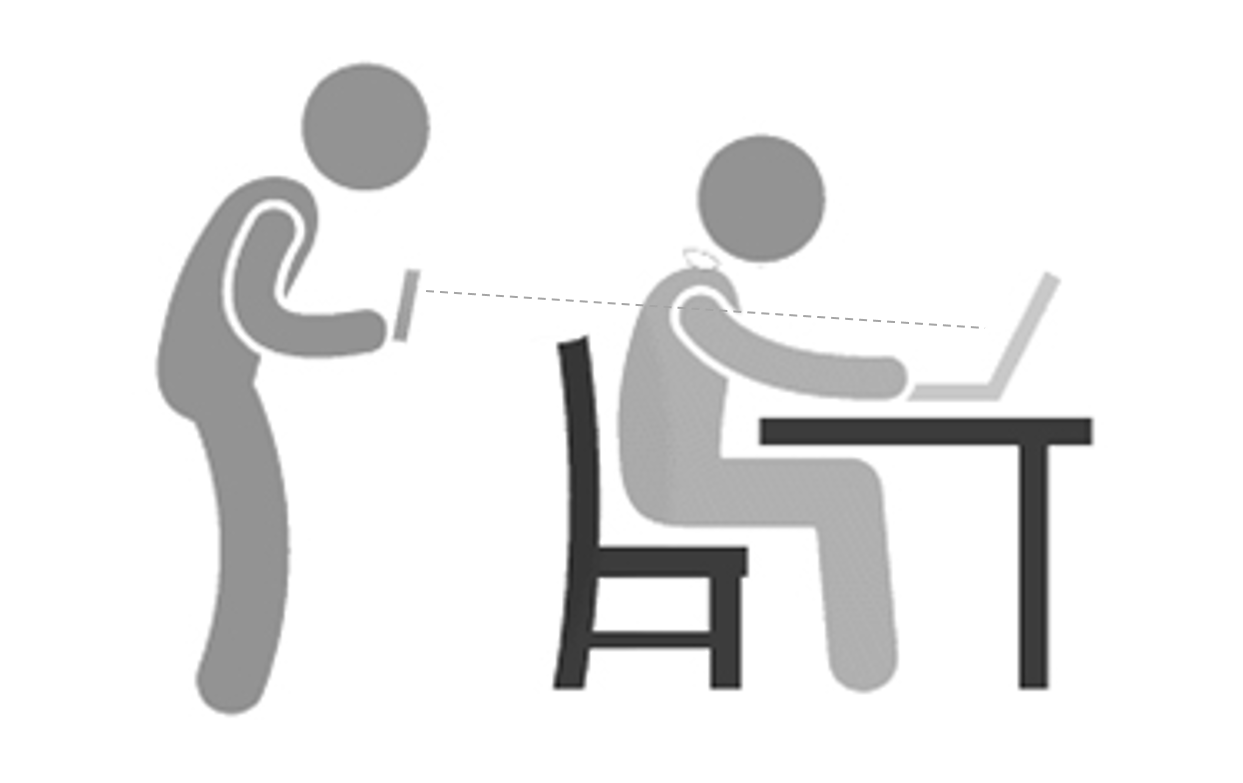
\includegraphics[width=0.48\textwidth]{pic/intro.png}
    \caption{Illustration of the long-range shoulder surfing threat model on smartphones, exacerbated by the SR algorithm. \cl{supplement elements for long range, blurred input and the recognized results.}}
	\label{illustration_of_system}
\end{figure}

\vspace{1mm}
\noindent
\textbf{Threat Model.} We present \textsf{SRPeek}, an end-to-end system of shoulder surfing using the SR algorithm, illustrated in Figure~\ref{illustration_of_system}. 
Assuming the victim is scanning messages in life, the attacker can raise his commercial smartphone with powerful lenses and our SR network to the victim stealthily, even from a long range (e.g., 1.5 meters far away within the visual angle of 30$^{\circ}$). As the camera zooms in, he can take 20 to 30 snapshots continuously in burst mode, with about 0.05 ~ 0.1 seconds of interval between frames. This process can take about 2 seconds with the consistent content and position for the screen of the victim. Benefited from our multi-frame SR neural network, those blurred snapshots can be then aligned, cropped, and processed, delivering a holistic threat model for acquisition of high-resolution contents of the victim in real time. Note that multi-type contents can be recovered accurately on the smartphone screen of the victim, covering numbers, English and Chinese characters. The above procedure can be automated by an app and repeated every few seconds, giving the attacker a continuous surveillance over the victim’s screen.

\vspace{1mm}
\noindent
\textbf{Challenges.} Creating a high-resolution shoulder surfing threat model, however, is not trivial, especially for commercial smartphones in real time. And we achieve \textsf{SRPeek} by overcoming four key challenges.

% \begin{figure}
% 	\centering
% 	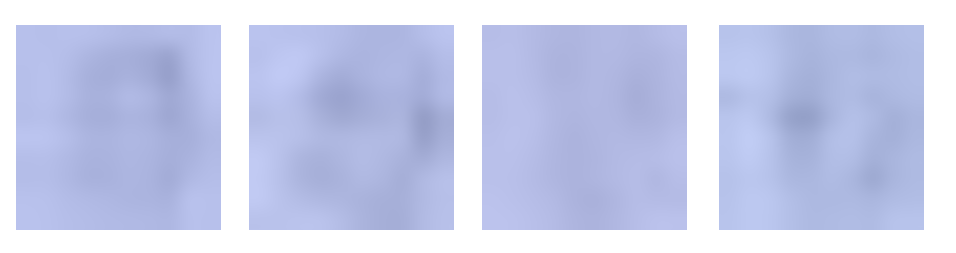
\includegraphics[width=0.48\textwidth]{pic/zeros.png}
%     \caption{Photos of number ‘0’ on a screen at a distance of 1.5m, taken in quick succession from a still smartphone camera. All exhibit different blurriness and no consistency between neighboring frames.\cl{Figure should be replaced.}}
% 	\label{illustration_of_system}
% \end{figure}

\begin{itemize}[leftmargin=*]
  \item \textbf{Blurriness of input images.} The most prominent one is the blurriness of captured snapshots, as they are taken secretly and hurriedly at extreme range, without much room for focusing. It can be further exacerbated by straining the magnification of the smartphone lenses. Unlike most SR applications and datasets working with ``normally" captured photos (e.g., scenery, scanned images) \cite{nasrollahi2020deep,lyn2020image}, images we face exhibit lower concentrations of information and more artifacts, and needs reliable ``reconstruction" than ``interpolation"". Since blurrier input means less information, rendering a greater possibility of reconstructing the wrong character. 
  % In deep learning based methods, a deep network often leads to gradual divergence from the truth as the data is propagated deeper through the network pipeline, resulting in 'fake' high-res images, especially when the subjects are the discrete strokes of characters, instead of details and texture of everyday objects. As a matter of fact, most works on multi-frame SR function on video clips \cite{lucas2019generative} or multiple snapshots \cite{wronski2019handheld}, however, our application is subtly different from the two. 
  On one hand, each photo is blurred with a randomly different PSF kernel, which, because of the extreme blurriness, cannot be approximated as a constant, isotropic gaussian kernel. Thus they cannot be processed as a video clip due to the lacking consistency between neighboring frames\cl{citation?}, shown in Figure~\ref{illustration_of_system}; on the other hand, because of the low concentration of information, blurred photos are similar to pieces of a jigsaw puzzle, each containing only fractions of information.
  % and the only chance of recovering the ground truth is to compare each photo against others. 
  Few useful information can be extracted separately and merged directly to produce satisfactory results if processed by common procedures to enhance the resolution of a series of snapshots\cl{citation?}. 
  \item \textbf{Super resolution with multiple frames.} To resolve the blurriness of input images, a SR algorithm on a smartphone is required to recover the captured contents. However, none of existing SR algorithms can be adapted for this attack scenario, especially with massive extremely blurred photos as input. Since smartphones can capture 10 snapshots per second in burst mode. Specifically, the difference between videos and multiple snapshots rules out existing image/video super resolution algorithms\cl{citation?}. The reason has two folds. First, either increased input leads to increases in model complexity, making it unsuitable for mobile deployment. Second, the nature of our task requires to do pixel-wise correlation and comparison with same coordinates on consecutive images throughout our construction process. Otherwise we cannot tell if, for example, it is one stroke or two parallel strokes that is shown in these two darker pixels on this photo.
  \item \textbf{Model complexity and variable input.} We have to operate our threat model locally on commercial smartphones in a real-time manner rather than remotely in cloud server. Since 1) the latter would require stable Internet access, and 2) sending multiple images across the Internet will consume time and bandwidth. Given the required 10 to 20 images to process for ideal content recovery, we have 1-2s as the minimum interval between each output frame, rendering limited period for calculation with restricted power and RAM. In cases where the display on the target screen changes more frequently, less images and processing time are available for each scene. Consequently, it cannot only require a smaller and simpler network model, but also a model that can deal with dynamic inputs efficiently, either 3 or 20 images.
  \item \textbf{Complexities of characters.} To deploy our threat model broadly for real-life scenarios (e.g., record passwords or e-mails), it is supposed to reconstruct multi-type texts, including Chinese characters, English letters, and numbers. Composed of multiple strokes, characters are distributed discretely in the pixel-wise image and different with other entities (e.g., faces and natural objects), rendering unique challenges. In some cases, messing up a stroke even slightly can shorten or lengthen a stroke, leading to a different character for misunderstandings. Unlike most SR applications working on similarity between their output and the ground truth, our network architecture and training process must be engineered to recover readable contents. Another challenge is the imbalanced element for words. Since we know certain stroke or alphabet of Chinese and English characters can occur more frequently, results in lower prediction accuracy over the less common, unconventionality shaped characters.
\end{itemize}

\vspace{1mm}
\noindent
\textbf{Summary of Evaluation Results.}
Equipped with our uniquely designed SR algorithm, our system can help the attacker read the characters shown on the victim's phone with above 90\% accuracy at 2m distance on a smartphone without optical zooming, or 6m distance on a phone with optical zooming in our experimental settings. The system is able to capture photos and produce high-res images constantly with about 2 seconds interval. Our experiments with real life scenarios show that this system is able to decipher texts or passwords of the victim at a safe distance, without alarming the victim, posing a threat to screen privacy.

\vspace{1mm}
\noindent
\textbf{Contributions.} This paper makes the following contributions:
\begin{itemize}[leftmargin=*]
  \item	We propose \textsf{SRPeek}, an end-to-end threat model of shoulder surfing from a broad range. To the best of our knowledge, we are the first to consider the presence of smartphone cameras and SR algorithms in shoulder surfing scenarios.
  \item	We design a multi-frame SR neural network architecture aiming at reconstructing extremely massive blurred and defocused snapshots. It can be further extended to other text-recognition applications on commercial smartphones.
  \item	We evaluate this new shoulder surfing attack in comprehensive scenarios. And it outperforms the state-of-the-arts for the new privacy concern.
\end{itemize}
% describe the organization of the paper
The rest of the paper is organized as follows. Section~\ref{sec-related-work} describes the related work, especially the state-of-the-arts for the shoulder surfing attack. We present the system and network design in Section~\ref{sec-design}, followed by the implementation and evaluation in Section~\ref{sec-implementation-and-training} and~\ref{sec-evaluation}, respectively. We further wrap up this paper by presenting the limitations and countermeasures of our system in Section~\ref{sec-limitations-and-discussions}. And the conclusion is show in Section~\ref{sec-conclusion}.
